\chapter{Informační systém pro správu závěrečných prací}

Úkolem praktické části bakalářské práce bylo provést analýzu a vytvořit grafickou podobu informačního systému  pro správu zadání, kontrolu a schvalování závěrečných prací vypsaných na partnerských fakultách společnosti Red~Hat.

Tvorbu praktické části práce jsem rozdělil do tří částí. Cílem první čísti bylo vytvořit drátěný model aplikace, který pomohl blíže specifikovat nástroje systému. Ve druhá části jsem se pustil do tvorby grafického návrhu, jehož úkolem bylo představit vizuální podobu aplikace. Úkolem poslední části bylo integrovat grafický návrh do implementace informačního systému.

\section{Popis požadavků na systém}

Informační systém poskytuje rozhraní pro studenty, kteří se mohou přihlašovat k tématům, komentovat jednotlivá témata nebo závěrečné práce. Dále k systému přistupují vedoucí, kteří mají ve správě témata, závěrečné práce a mohou schvalovat přihlášky studentů přihlášených k tématům. Systém poskytuje rozhraní i pro návštěvníky, kteří mohou procházet jednotlivá témata a závěrečné práce. Studenti partnerských fakult se mohou zaregistrovat na základě fakultního e-mailu.

Systém eviduje témata, závěrečné práce, uživatele, univerzity a přihlášky. Jednotlivá témata popisují cíl práce a mohou být vypsány pro více studentů. Systém umožňuje témata vypisovat, upravovat a mazat. Témata evidují:

\begin{itemize}
    \item seznam přihlášených studentů;
    \item seznam univerzit, na kterých je téma vypsáno;
    \item seznam externích a univerzitních vedoucích;
    \item typ tématu -- bakalářská nebo diplomová práce;
    \item seznam závěrečných prací, které byly na základě tématu vypsány.
\end{itemize}

Ke každé závěrečné práci se smí přihlásit pouze jeden student. Systém umožňuje práce vytvářet (na základě tématu), upravovat a mazat. Každá závěrečná práce eviduje:

\begin{itemize}
    \item studenta, který je k práci přihlášen;
    \item téma, ze kterého byla práce vypsána;
    \item univerzitního vedoucího práce;
    \item univerzitu, na které je práce vypsána;
    \item typ závěrečné práce -- bakalářská nebo diplomová práce;
    \item stav závěrečné práce -- přihlášená, dokončená, neúspěšná a odložená.
\end{itemize}

V systému existuje několik uživatelských rolí, které se liší v přístupových právech. Každý registrovaný uživatel je automaticky student. Systém eviduje následující uživatelské role:

\begin{description}
    \item[Návštěvník] Má právo procházet jednotlivá témata, závěrečné práce a registrovat se na základě fakultního e-mailu.
    \item[Student] Může se přihlásit k povoleným tématům, spravuje vlastní závěrečné práce, dále má možnost komentovat jednotlivá témata a závěrečné práce.
    \item[Univerzitní vedoucí] Jedná se o vedoucího na dané univerzitě, může závěrečné práce vytvářet a schvaluje přihlášky podané studenty k jednotlivým tématům.
    \item[Vedoucí] Na rozdíl od univerzitního vedoucího patří pod jeho správu i tvorba zadání témat.
    \item[Správce] Může spravovat většinu obsahu, přidávat do systému univerzity a uživatele.
\end{description}

%new
\section{Plánování a analýza}

V rámci tvorby uživatelského rozhraní bylo nutné provést analýzu a porozumět požadavkům kladeným na funkční celky systému. Aby se tedy vývoj systému ubíral správným směrem, bylo nutné pravidelně komunikovat s klientem. Cílem prvních fází tvorby rozhraní byl sběr informací, neboť na základě jejich vyhodnocení mohla být poskytnuta první odezva -- je-li například možné některé požadavky realizovat, je-li jejich realizace praktická a případně existuje-li efektivnější alternativa.

\subsection{Analýza nástrojů systému}

Pro zvýšení kvality uživatelského rozhraní jsou podstatné i další prvky, které nemusí být příliš prioritní a uživatele tolik neomezují. Jejich existence však vede k rychlejší orientaci a často zvyšuje používanost systému.
Během sběru informací a konzultací s klientem tak vznikl seznam další nástrojů, které byly v systému použity. Tyto nástroje mají za cíl zvýšit kvalitu UX designu.

\begin{description}
    \item[Kategorie a štítky] Použití štítků umožňuje uživatelům snadněji třídit témata a závěrečné práce. Jeden z prvních nápadů integrace štítků do systému bylo umožnit jejich standardní přiřazování k jednotlivým tématům, avšak s nutností hierarchického zařazení pod některý z kořenových štítků. Kořenové štítky by představovaly kategorie a mohl by je vytvářet pouze správce, zatímco standardní štítky by vytvářeli vedoucí a studenti. Tento přístup má však několik nevýhod -- prvním problémem je netradiční a tím pádem poměrně neintuitivní způsob použití, další potíž je nutnost vyšší organizace a správy. Nakonec jsem se rozhodl integrovat štítky v systému standardním způsobem a používat je odděleně s kategoriemi.
    \item[Komentáře] Možnost přispívat k jednotlivým tématům snižuje nutnost e-mailové korespondence a zároveň poskytuje rozhraní pro obecné dotazy. Aby bylo docíleno vyšší použitelnosti, lze v systému psát komentáře s využitím syntaxe Markdown.
    \item[Odevzdávárna souborů] Pro jednoduchou manipulaci s přílohou závěrečné práce je vhodná odevzdávarna, která je určená pro nahrávání závěrečného textu a dalších materiálů použitých v praktické části práce.
    \item[Filtry] Využití filtrů umožňuje témata třídit nejen podle štítků, ale také podle vedoucích a univerzit.
    \item[Notifikace] Pokud vedoucí například schválí přihlášku studenta nebo napíše komentář k závěrečné práci, je příhodné jej na tuto akci upozornit. Notifikace představují oznámení, které uživatele informují o související aktivitě v sytému.
\end{description}
%new

\subsection{Analýza cílové skupiny}

Cílová skupina uživatelů pracující se systémem je velice úzce zaměřená. Největší část návštěvníků tvoří studenti z technicky zaměřených oborů. Tato skupina je dána typem závěrečných prací, pro které je systém primárně určen -- jedná se o témata z IT oboru. K systému navíc přistupují především studenti v posledních ročnících bakalářského nebo magisterského studia a jejich vedoucí. Tyto skutečnosti mi dávají větší \uv{svobodu} při volbě technologií pro integraci grafického návrhu.

\section{Základní layout}

Rozhodl jsem se vytvořit a používat v aplikaci pouze tři základní layouty, přičemž dva se liší pouze prohozením postranního panelu a obsahové části. Použití příliš velkého množství variant uspořádání komponent stránky může snižovat použitelnost, naopak volba pouze jednoho layoutu působí příliš staticky. Primární layout (obrázek \ref{img:layout1}) tvoří:

\begin{itemize}
    \item Navigační panel -- nachází se v záhlaví stránky a obsahuje hlavní informace o přihlášeném uživateli, vyhledávač a logotyp.
    \item Navigační menu -- slouží jako primární navigace na stránce.
    \item Levý sloupec -- je určen pro seznam a popis témat, závěrečných prací, jejich primární popis i anotaci. Dále může obsahovat odevzdávárnu souborů a komentáře.
    \item Pravý sloupec -- slouží jako přehled informací o daném tématu nebo dané závěrečné práci. Dále může obsahovat nástroje pro správu závěrečných prací (popř. témat) nebo filtry.
\end{itemize}

Sekundární layout představuje kostru profilu uživatelů a univerzit. Na rozdíl od primárního layoutu je sloupec s vedlejším obsahem přemístěn na levou část stránky. Tvoří ho:

\begin{itemize}
    \item Navigační panel a navigační menu.
    \item Levý sloupec -- obsahuje podrobnější informace o uživateli včetně profilového obrázku.
    \item Pravý sloupec -- slouží jako obecný přehled vedených závěrečných prací, vlastních prací a aktivity uživatele v systému.
\end{itemize}

Poslední layout je speciálně navržený pro formuláře (např. formulář pro vytváření závěrečných prací nebo témat). Obsahuje pouze nejnutnější prvky aplikace a je tvořen z jednoho sloupce:

\begin{itemize}
    \item Navigační panel.
    \item Hlavní sloupec -- určený pro formulářová pole.
\end{itemize}

V systému figuruje ještě jeden odlehčený layout, který je určen pouze pro autentizaci uživatele. Minimální šířka všech stránek je $1040~px$ -- při nižších hodnotách je uživatel nucen horizontálně skrolovat. Tuto šířku jsem zvolil s ohledem na aktuální podíl populárních rozlišení monitorů, který v současnosti z více než $90~\%$ tvoří rozlišení větší než $1024\times768~px$\footnote{\url{http://gs.statcounter.com/\#resolution-CZ-monthly-201203-201303}}.

\begin{figure}[htbp]
    \centering
    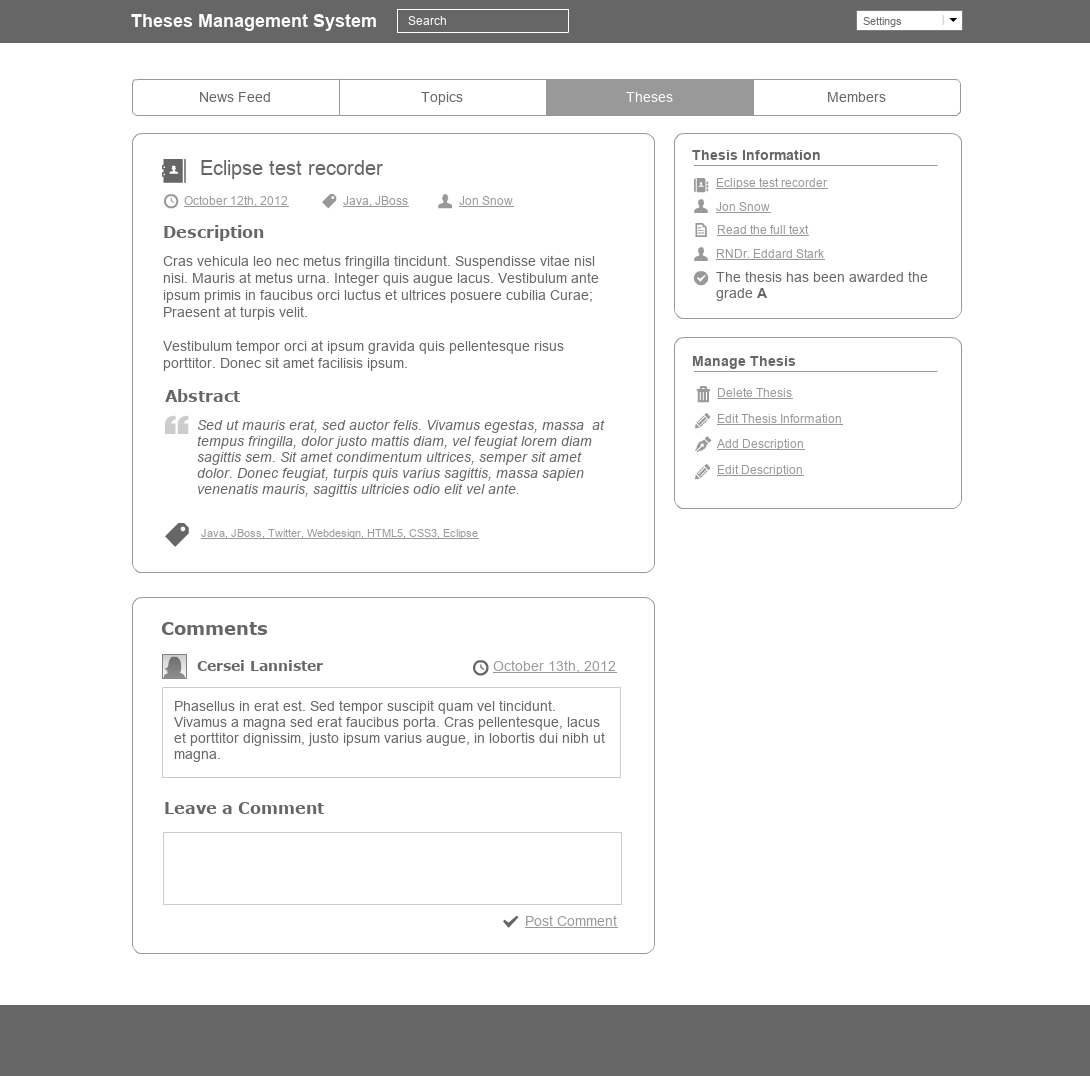
\includegraphics[width=\textwidth]{images/w1.png}
    \caption{Výsledný drátěný model profilu diplomové práce.}
    \label{img:layout1}
\end{figure}

\section{Grafický návrh}

Přesto, že nebyly kladeny žádné nároky na dodržení vizuálního stylu společnosti Red Hat, rozhodl jsem se z něj čerpat alespoň částečně především co se týče barevnosti. Zatímco tvorba drátěného modelu je důležitá převážně pro zvýšení použitelnosti systému, vývoj grafického návrhu zahrnuje především aktivity spojené s UI designem.

\subsection{Písmo}

Ještě relativně nedávno byly designeři při volbě písma pro webové aplikace omezeni na několik málo základních fontů, které byly přítomny na klientských počítačích -- mezi něž patří například Arial, Times New Roman, Georgia nebo Courier Sans. Díky novému CSS~3 pravidlu \texttt{@font-face} je však toto omezení minulostí a nyní je možné používat i fonty, které nejsou na klientských počítačích nainstalovány.

Již na počátku tvorby jsem se rozhodl používat pro nadpisy lineárně serifové písmo s rovnými serify\footnote{Viz klasifikace písma podle Jana Solpery.}. Volba písma byla poměrně omezená především pro nutnost podpory české znakové sady. První volbou bylo písmo Sanchez\footnote{\url{http://www.myfonts.com/fonts/latinotype/sanchez/}} od designéra Daniela Hernándeze, které jsem však později zavrhl z důvodu špatné optimalizace pro webové prohlížeče. Nakonec jsem zvolil písmo Museo Slab\footnote{\url{http://www.myfonts.com/fonts/exljbris/museo-slab/}}, které navrhl designér Jan Buivenga.

\begin{figure}[htbp]
    \centering
    \includegraphics[width=\textwidth]{images/museo.pdf}
    \caption{Museo Slab 500}
    \label{img:museo}
\end{figure}

Jako primární písmo jsem se rozhodl použít velmi rozšířený Arial. Jedná se o bezpatkový grotesk, který je již od počátku součástí všech verzí Microsoft Windows. Arial bývá často kritizován pro svou podobnost s Helveticou, přesto se však jedná o velmi dobře čitelný a vysoce optimalizovaný font.

\subsection{Piktogramová řada}

Jako sadu ikonek jsem zvolil Font Awesome\footnote{\url{http://fortawesome.github.io/Font-Awesome}}, který byl primárně navržen pro integraci s webovým rámcem Twitter Bootstrapem. Samotná piktogramová řada je licencována pod CC BY 3.0, je tedy možné používat samotnou řadu odděleně.

\subsection{Typografie}

Jako základní velikost písma jsem zvolil $16~px$, díky čemuž je text dobře čitelný i na monitorech s vyšším PPI. Vzhledem k větší střední výšce písma Arial jsem se rozhodl zvýšit hodnotu řádkového prokladu, aby i rozsáhlejší části textu nepůsobily příliš sevřeně.

Nadpisy první až čtvrté úrovně jsou vysázeny písmem Museo Slab s maximální velikostí $34~px$, která je užita výhradně pro název témat a závěrečných prací.

Jako velikost okrajů primárního sloupce s obsahem jsem se rozhodl zvolit $30~px$, čímž je zajištěn dostatečný prostor pro jednoduchou orientaci mezi odstavci a jsou tak jasně odlišeny bloky textu.

\subsection{Barevnost}

Vizuální styl společnosti Red Hat se orientuje v barvách bílé, černé a červené. Rozhodl jsem se použít světlejší barvy pro navození klidnějšího dojmu a snížení kontrastu, neboť příliš vysoký kontrast může působit dráždivě a není podle mě příliš vhodný pro systém určený primárně pro správu závěrečných prací.

V grafickém návrhu je použito osm stupňů šedi a dva stupně červené barvy. Několik dalších barev jsem použil výjimečně například pro zvýraznění aktivních kategorií nebo pro systémové zprávy a upozornění.

\begin{figure}[htbp]
    \centering
    \includegraphics[width=\textwidth]{images/barvy.pdf}
    \caption{Základní barvy používané v grafickém návrhu.}
    \label{img:colors}
\end{figure}

\begin{figure}[htbp]
    \centering
    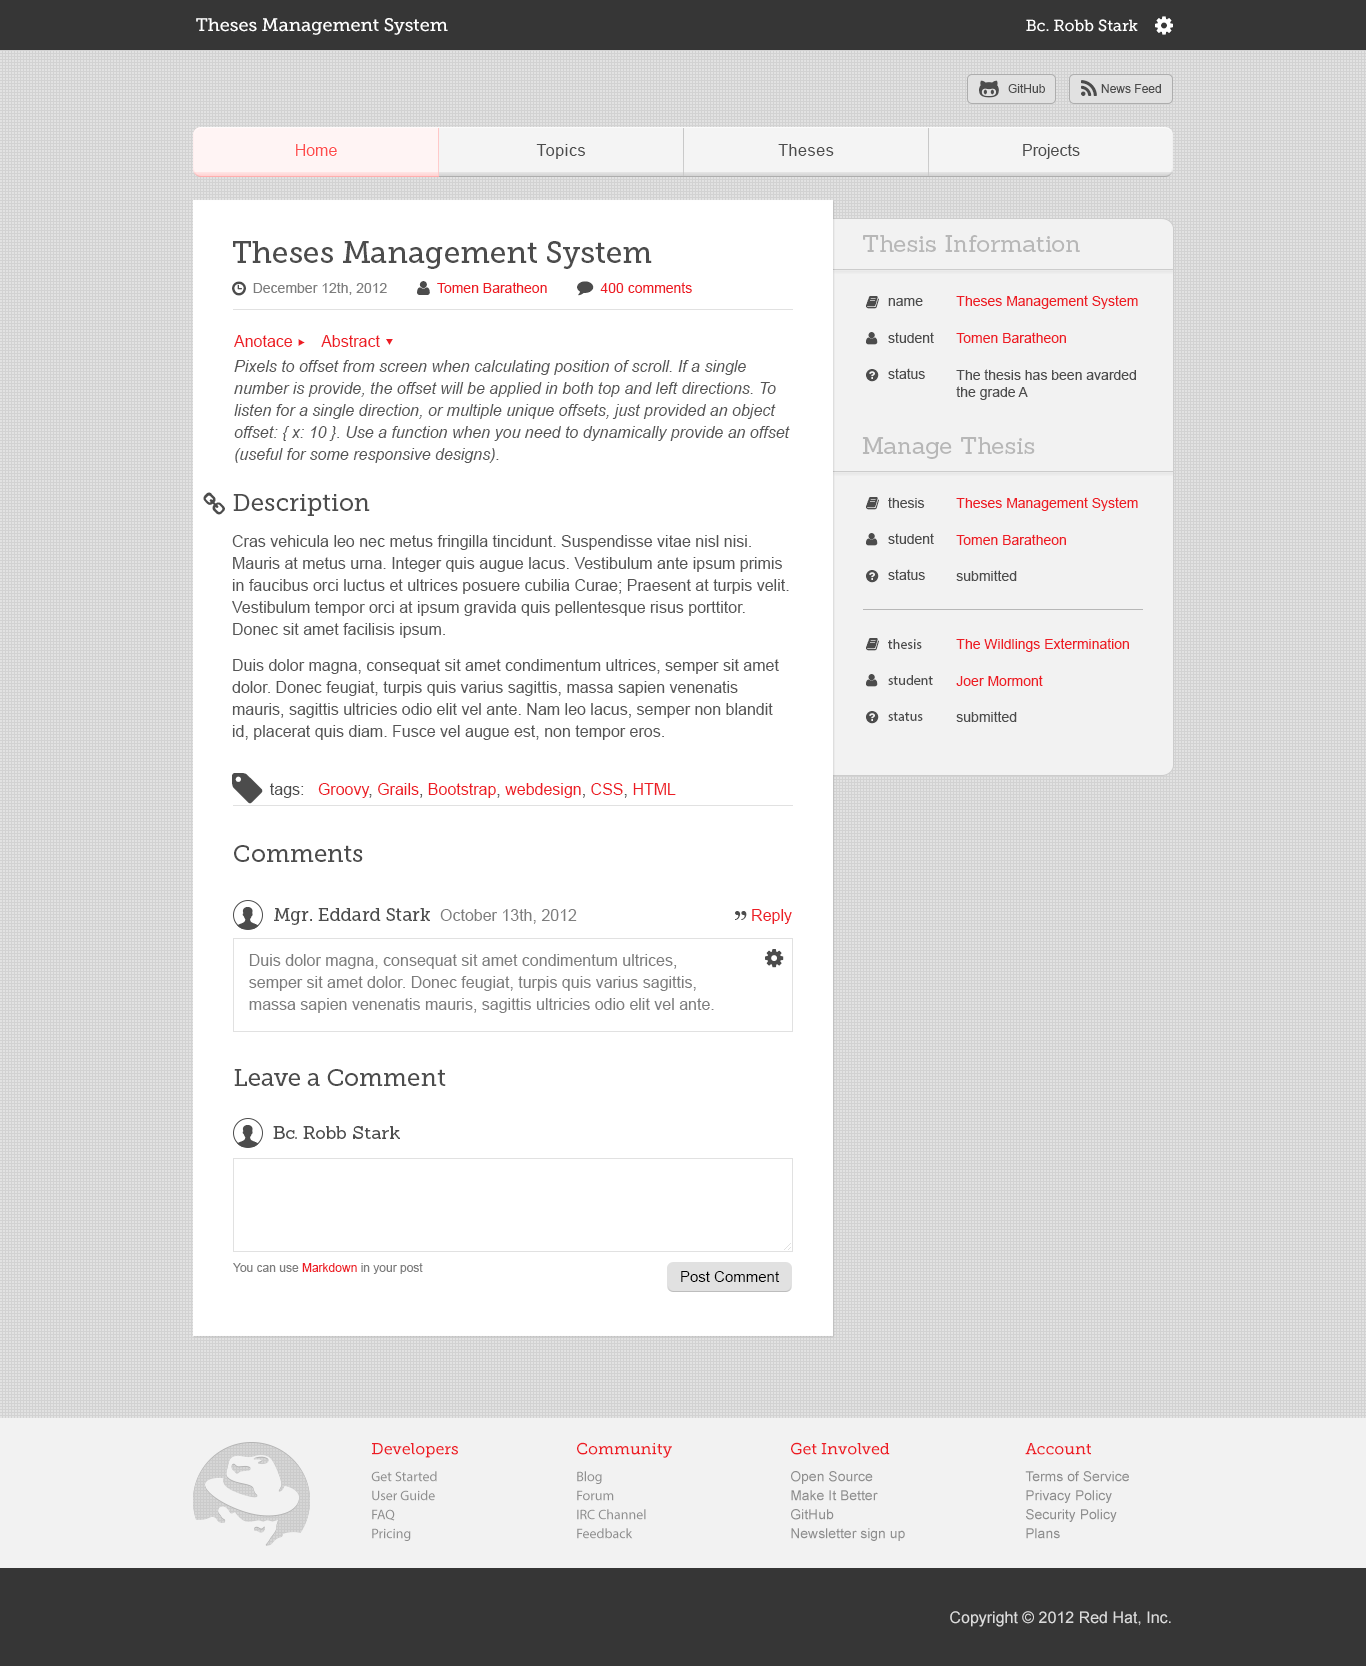
\includegraphics[width=\textwidth]{images/gd1.png}
    \caption{Výsledný grafický návrh profilu diplomové práce.}
    \label{img:design}
\end{figure}

\section{Integrace návrhu}

Prezentační vrstva systému využívá následující technologie, knihovny a webové rámce:

\begin{itemize}
    \item HTML~5 (viz kapitola~\ref{sec:html})
    \item CSS~3 (viz kapitola~\ref{sec:css})
    \item LESS (viz kapitola~\ref{sec:less})
    \item JavaScript
    \item Twitter Bootstrap (viz kapitola~\ref{sec:bootstrap})
    \item GSP (viz kapitola~\ref{subsec:gsp})
\end{itemize}

Nadměrné použití některých technologií (typicky JavaScriptu) přitom může vést ke snížení použitelnosti systému, je tedy důležité zvážit jejich využití.

Zatímco ve čtvrté kapitole jsem se věnoval specifikaci několika výše jmenovaných technologií, nyní se zaměřím na jejich použití v informačním systému. Vzhledem k zaměření systému však není potenciál všech použitých technologií plně využit (jde zejména o HTML~5 standard).

\subsection{HTML~5}

Velká část HTML~5 je v současné době všemi moderními prohlížeči podporována a je tak již možné mnoho novinek volně používat. Aplikace implementuje v zásadě jen některé nové HTML~5 atributy a sémantické elementy. V budoucnu je však možné aplikaci rozšířit o další novinky, které tento nový standard přináší.

\subsection{CSS~3}

Nové vlastnosti a selektory využívám v systému hojně, neboť umožňují jednak velkou část webu vytvořit bez použití rastrových obrázků, dále zvyšují čistotu kódu a pomáhají zachovat jednoduchost stránky z hlediska její struktury.

Mezi jednu z předních výhod CSS~3 patří revoluce v podobě pravidla \texttt{@font-face}, která umožňuje definici vlastních fontů. Tímto je zároveň umožněno použití sady piktogramů ve formě fontu, díky čemuž odpadá nutnost práce s rastrovou sadou ikonek. Nové vlastnosti uplatňuji užitím fontu Awesome jako sady piktogramů a fontu Museo Slab pro čtyři úrovně nadpisů.

\begin{demo}
    \centering
    \begin{lstlisting}[language=css]
/* Definice ikonky v CSS */
.icon-rss:before { content: "\f09e"; }
    \end{lstlisting}
    \begin{lstlisting}[language=html5]
<!-- Pouziti ikonky v HTML dokumentu -->
<i class="icon-rss"></i>
    \end{lstlisting}
    \caption{Použití fontu Awesome.}
    \label{demo:awesome}
\end{demo}

\subsection{Twitter Bootstrap}

Díky Twitter Bootstrapu je návrh jednotlivých HTML dokumentů konzistentní a lépe udržovatelný. Zároveň je docíleno vyšší podpory Internetovými prohlížeči, přičemž jsou snáze dodržovány osvědčené postupy a doporučení.

Použití Bootstrapu mě zbavilo nutnosti trávit nepřiměřené množství času optimalizací aplikace pro webové prohlížeče, zároveň mi rámec nabídl mnoho nástrojů a předdefinovaných komponent, které urychlili vývoj prezentační vrstvy aplikace.

Grafický návrh systému se značně liší od vizuálního stylu Bootstrapu, bylo tedy potřeba některé součásti upravovat. Stejný úmysl je běžný pro mnoho aplikací, které používají nějaký webový rámec pro tvorbu uživatelského rozhraní. S tímto problémem se lze vypořádat částečnou úpravou zdrojového kódu webového rámce podle vlastních potřeb. Takový postup však není doporučován, neboť znemožňuje rámec později jednoduše aktualizovat (bez použití nějakého verzovacího systému). Rozhodl jsem se tedy pro řešení, které znázorňuje adresářová struktura na obrázku \ref{fig:tree}, kde:

\begin{itemize}
    \item adresář \texttt{bootstrap} obsahuje zdrojové soubory Bootstrapu;
    \item soubor \texttt{bootstrap.less} obsahuje importy použitých komponent Bootstrapu a vlastní definované kaskádové styly (importy vlastních stylů musí být umístěny na konci souboru);
    \item soubor \texttt{variables.less} je určen pro deklaraci proměnných;
    \item soubor \texttt{main.less} slouží pro definici vlastních stylů.
\end{itemize}

\begin{figure}
    \dirtree{%
    .1 web-app.
    .2 less.
    .3 bootstrap.
    .4 alerts.less.
    .4 ....
    .3 bootstrap.less.
    .3 variables.less.
    .3 main.less.
    .3 ....
    }
    \caption{Stromová struktura adresáře ve kterém jsou obsaženy kaskádové styly používané v aplikaci.}
    \label{fig:tree}
\end{figure}

\subsection{LESS}

Použití preprocesoru LESS zpřístupnilo mnoho konstrukcí, které z důvodu zachování formální čistoty jazyka v CSS chybí. Díky LESS je psaní stylů přehlednější, kratší a organizovanější. Chceme-li například změnit barvu odkazů nebo odstranit podtržení, stačí tak učinit na jediném místě v kódu.

Pro eliminaci neúmyslného přepsání kaskádových stylů, které jsou součástí Bootstrapu jsem zavedl konvenci pro pojmenování vlastních tříd a identifikátorů. Každá třída, která není součástí Bootstrapu obsahuje prefix \texttt{tms-}, tedy například tlačítka jsou v systému označovány třídou \texttt{.tms-btn}, naopak v Bootstrapu pouze \texttt{.btn}.

Vlastní kaskádové styly jsou deklarovány v souborech:

\begin{itemize}
    \item \texttt{main.less} -- soubor určený pro formátování elementů a definici maker, proměnné jsou deklarovány v souboru \texttt{variables.less}, který je přejatý od Bootstrapu;
    \item \texttt{fonts.less} -- definice fontů používaných v aplikaci (daklarovány pravidlem \textit{@font-face});
    \item \texttt{taggy.less} -- kaskádové styly přídavného modulu pro podporu štítků\footnote{Štítky jsou klíčové slova, které identifikují závěrečnou práci nebo téma. Štítky jsou užitečné například při vyhledávání.};
    \item \texttt{fineuploader.less} -- kaskádové styly přídavného modulu pro podporu nahrávání souborů.
\end{itemize}

\subsection{GSP}
\label{subsec:gsp}

Hlavní funkce systému jsou napsány v programovacím jazyce Groovy za použití platformy Grails. Jako výchozí jazyk pro popis prezentační vrstvy aplikace používá tato platforma GSP (\textit{Groovy Server Pages}). Jedná se o jazyk inspirovaný JSP (\textit{JavaServer Pages}) speciálně navržený pro dynamické zpracování HTML dokumentů.  \cite{20}

GSP umožňuje aplikovat dynamické chování dokumentu jednak zasazením samotného Groovy kódu do bloků \texttt{<\% ... \%>} (jedná se však o nedoporučený postup) nebo použitím GSP elementů. V prezentační vrstvě používám výhradně druhý způsob. Jako největší nevýhodu této strategie považuji jeho poměrně vysokou nepřehlednost.

Na ukázce \ref{demo:parent} (nahoře) lze vidět příklad GSP stránky, která slouží jako layout pro tzv. \uv{potomky} (t.j. stránky, které tento definovaný dokument rozšiřují).

\begin{demo}
    \centering
    \begin{lstlisting}[language=html5]
<!-- parent.gsp -->
<!DOCTYPE html>
<html>
    <head>
        <title><g:layoutTitle /></title>
        <g:layoutHead />
    </head>
    <body>
        <div class="span9">
            <g:layoutBody />
        </div>
    </body>
</html>
    \end{lstlisting}
    \begin{lstlisting}[language=html5]
<!-- child.gsp -->
<!DOCTYPE html>
<html>
    <head>
        <meta name="layout" content="parent">
        ...
    </head>
    <body>
        ...
    </body>
</html>
    \end{lstlisting}
    \caption{Rodič (nahoře) a potomek (dole).}
    \label{demo:parent}
\end{demo}

Každý potomek je definován uvedením rodiče v hlavičce dokumentu, přičemž na místo elementu \texttt{<g:layoutBody/>} je vykresleno tělo potomka, element \texttt{<g:layoutHead/>} je nahrazen hlavičkou a \texttt{<g:layoutTitle/>} titulkem potomka.

\begin{figure}[htbp]
    \centering
    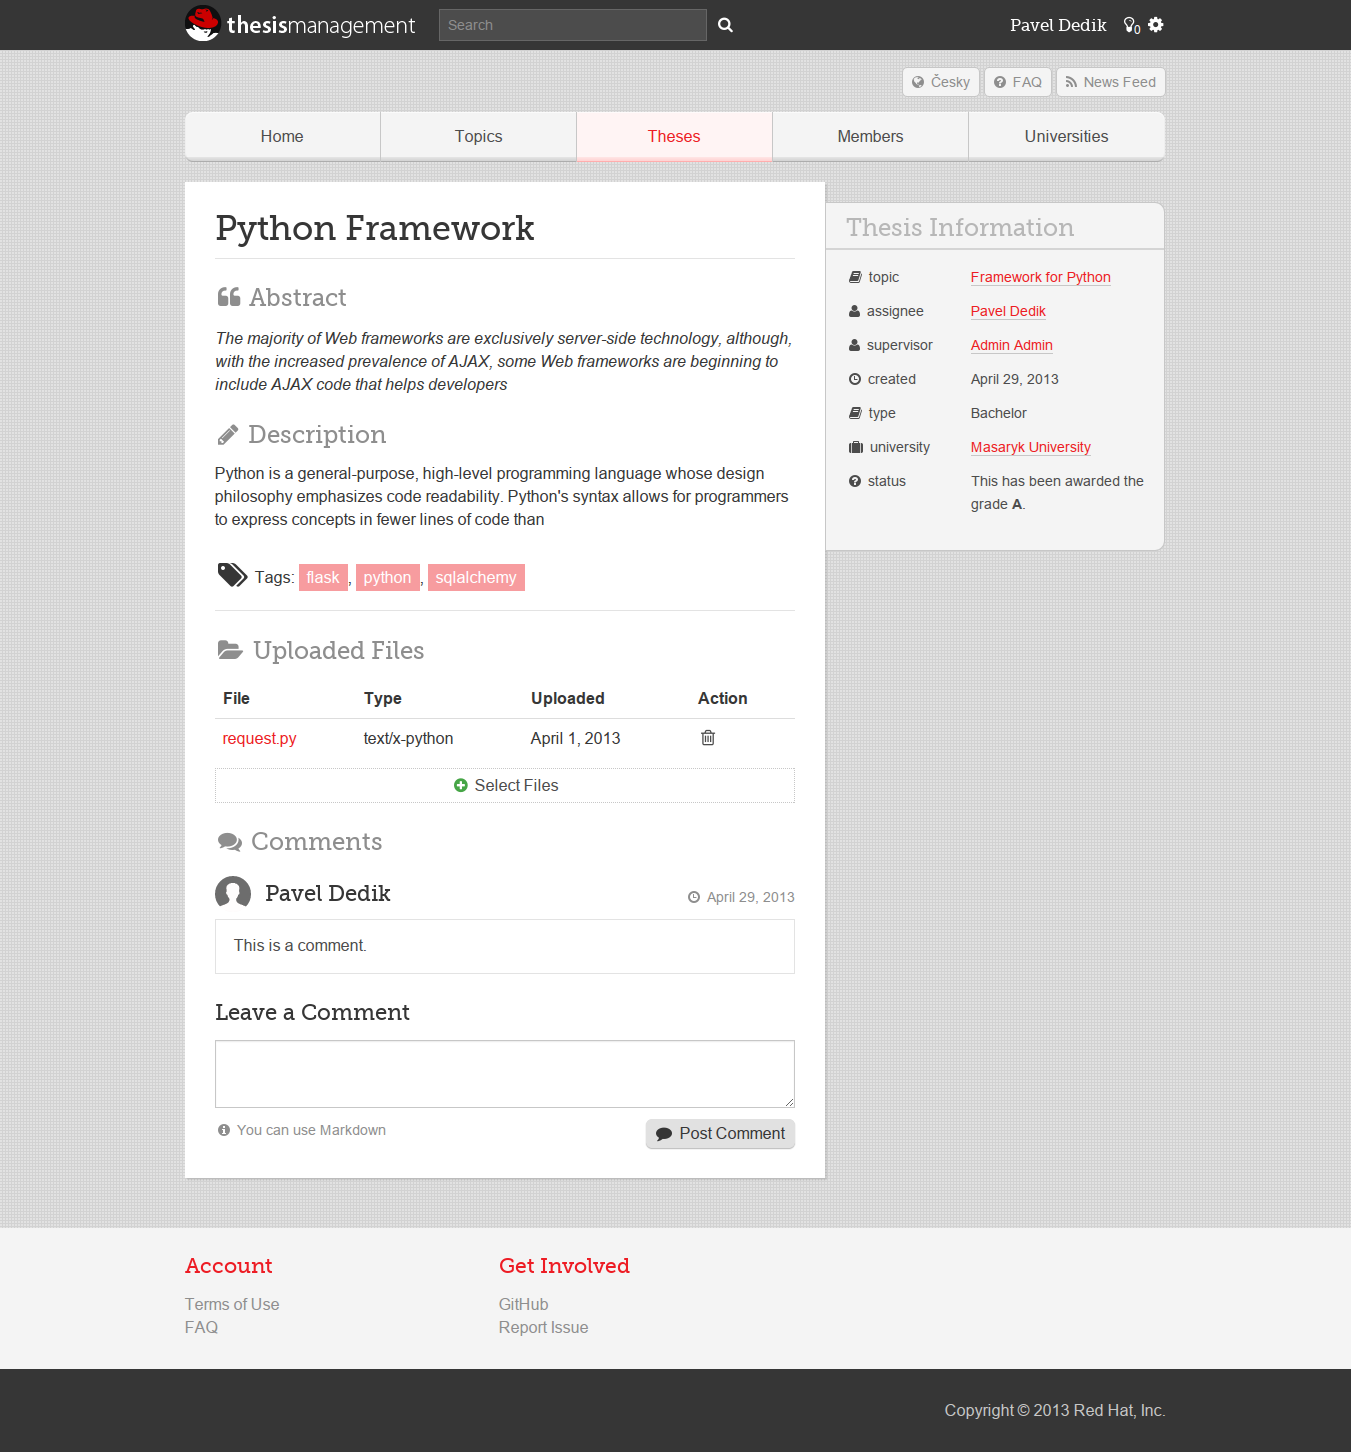
\includegraphics[width=\textwidth]{images/tms.png}
    \caption{Ukázka výsledné aplikace -- profil diplomové práce.}
    \label{img:tms}
\end{figure}
